\documentclass[a4paper]{memoir}
% This file needs to be compiled separately. LaTeX is not very good at mixing
% different typographic styles, which is needed for the frontpage. The solution
% presented here may not be the most elegant, but it definitely works.
% Set the name of your thesis or research assignment, your name, supervisors,
% report number etc. Then compile using
% pdflatex frontpage
% The generated pdf-file will then be included in the main document
\usepackage[utf8]{inputenc}
\usepackage[left=0mm,right=0mm,top=0mm,bottom=0mm]{geometry}
\usepackage{graphicx}
\usepackage{tikz}
\setlength\parindent{0pt}

\renewcommand\sfdefault{phv} % use helvetica for sans serif
\renewcommand\familydefault{\sfdefault} %use sans serif by default

\begin{document}

\begin{tikzpicture}[remember picture]
% Required to prevent LaTeX from doing all kinds of nasty things with margins
\path[use as bounding box,draw=none](0mm,-3.5mm) rectangle ++(0.001mm,0.001mm);

% NOTE: THIS IS THE OLD STYLE
% Include big logo
%\node[anchor=north east,inner sep=0pt] at (19.8,-1.2) {
\includegraphics[width=156mm]{frontpage/utewi}};

% NOTE: THIS IS THE NEW STYLE
% Include side bar (choose 1-5)
\node[anchor=north west,inner sep=0pt] at (-2,0) {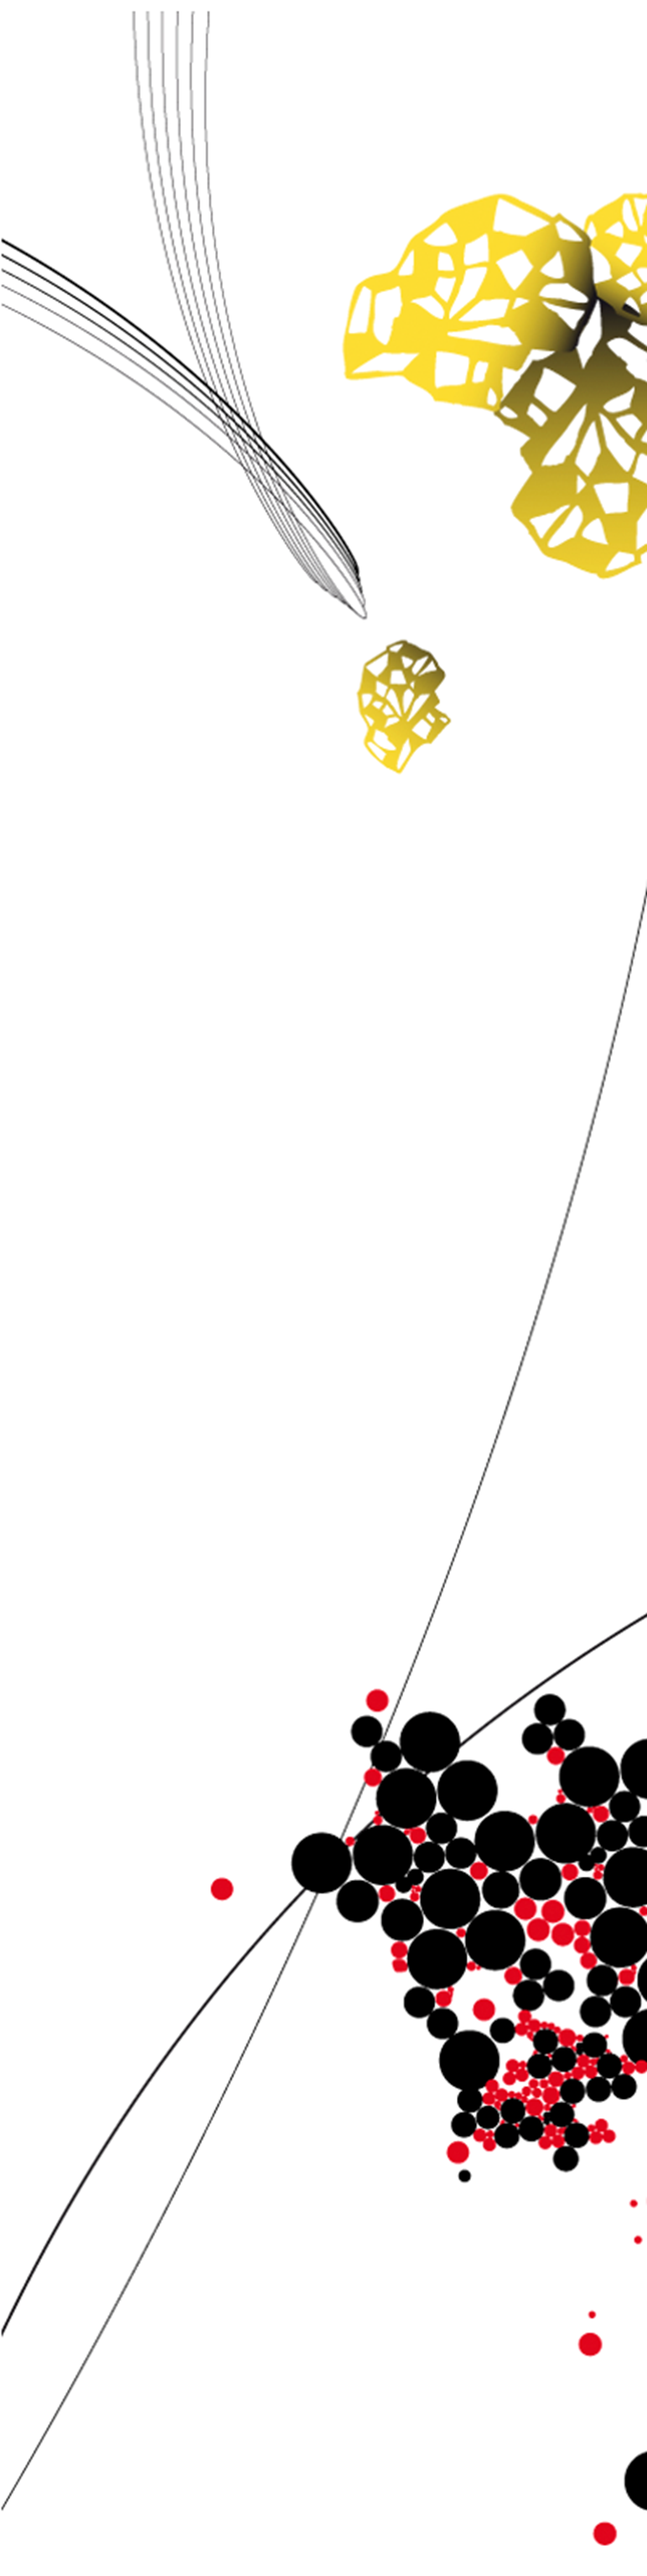
\includegraphics[height=297mm]{frontpage/sidebar3}};
% Include big logo
\node[anchor=north east,inner sep=0pt] at (20.7,-1.2) {
\includegraphics[width=150mm]{frontpage/ut}};

\node[anchor=north east,inner sep=0pt] at (19.8,-4.0) {
\begin{minipage}{15cm}
\begin{flushright}
\fontsize{18}{22}\selectfont
\textbf{Faculty of Electrical Engineering,\\Mathematics \& Computer Science}
\end{flushright}
\end{minipage}
};

% Title of the thesis. Change this to your title. You do not necessarily have
% to provide line breaks manually, but it usually looks better
\node[inner sep=0pt] at (13,-12.5) {
\begin{minipage}{20cm}
\begin{center}
\fontsize{25}{30}\selectfont
\textbf{Marrying GUI and Git:\\ How Authoring Tools\\ for E-Learning Can Benefit\\ from Version Control}
\end{center}
\end{minipage}
};

% Your name, type of document and date. Change this.
\node[inner sep=0pt] at (13,-18) {
	\begin{minipage}{20cm}
		\begin{center}
		\textbf{\Large{
		Simon Kreiser\\[1mm]
		M.Sc. Thesis\\[1mm]
		March 2016
		}}
		\end{center}
	\end{minipage}
};

% Supervisors, report number, etc. Change this.
\node[anchor=south east, inner sep=0pt] at (19.7,-28.7) {
	\begin{minipage}[r]{\textwidth}
		\flushright{
		\rule[0mm]{5cm}{.75mm}\\
		\textbf{Supervisors:}\\
		Dr. Mariët Theune\\
		Prof. Dr. Dirk Heylen\\
		Julian Ringel\\
		\vspace{\baselineskip} % empty line
		Human Media Interaction Group\\
		Faculty of Electrical Engineering,\\
		Mathematics and Computer Science\\
		University of Twente\\
		P.O. Box 217\\
		7500 AE Enschede\\
		The Netherlands \\}
		\rule[0mm]{5cm}{.75mm}
	\end{minipage}
};

\end{tikzpicture}
\end{document}
